\documentclass[a4paper, 12pt]{article}

\input{/home/nick/latex-preambles/xelatex.tex}

\setmainfont{Minion Pro}

\newcommand{\imagesPath}{.}

\title{
	\textbf{Εργαστήριο Δικτύων Υπολογιστών} \\~\\
	Εργαστηριακή Άσκηση 12 \\ 
	Υπηρεσίες στο Διαδίκτυο	
}
\author{}
\date{}

\begin{document}
\maketitle
\begin{center}
	\begin{tabular}{|l|l|}
		\hline
		\textbf{Ονοματεπώνυμο:} Νικόλαος Παγώνας, el18175  & \textbf{Όνομα PC:} nick-ubuntu \\
		\hline
		\textbf{Ομάδα:} 1 (Τρίτη 10:45) & \textbf{Ημερομηνία Εξέτασης:} Τρίτη 31/05/22 \\
		\hline
	\end{tabular}
\end{center}

\section*{Άσκηση 1: Εγκατάσταση DHCP server}
	
	Κατασκευάζουμε ένα εικονικό μηχάνημα με βάση ένα νέο FreeBSD 12.3 με \textbf{3} κάρτες δικτύου:
	
	\subsection*{1.}
		Ορίζουμε τη διεπαφή \verb|em1| σε NAT.
	
	\subsection*{2.}
		Εκτελούμε \verb|dhclient em1|.
	
	\subsection*{3.}
		Εκτελούμε \verb|ping www.google.com|. Το ping είναι επιτυχές.
	
	\subsection*{4.}
		Εκτελούμε \verb|pkg update|. 
	
	\subsection*{5.}
		Εκτελούμε \verb|poweroff| και ύστερα από τη διαδρομή File$\rightarrow$Export Appliance... δημιουργούμε ένα αρχείo \verb|new.ova|. \\
		
	Στη συνέχεια δημιουργούμε ένα νέο μηχάνημα NS1 βασισμένο στο \verb|new.ova|. 
	
	\subsection*{1.}
		Εκτελούμε \verb|pkg install isc-dhcp44-server|.
		
	\subsection*{2.}
		Κατασκευάζουμε ένα δικό μας \verb|dhcpd.conf| με περιεχόμενα:
		
		\begin{verbatim}
			default-lease-time 60;                            # (e)
			max-lease-time 120;                               # (f)
			
			subnet 192.168.2.0 netmask 255.255.255.240 {      # (a)
			  range 192.168.2.5 192.168.2.6;                  # (b)
			  option routers 192.168.2.1;                     # (c)
			  option broadcast address 192.168.2.15;          # (d)
			}
		\end{verbatim}
		
	\subsection*{3.}
		Εκτελούμε:
		
		\begin{verbatim}
			sysrc ifconfig_em0="192.168.2.1/28"               # (a)
			sysrc ifconfig_em1="DHCP"                         # (b)
			sysrc dhcpd_enable="YES"                          # (c)
			sysrc dhcp_ifaces="em0"                           # (d)
			sysrc hostname="ns1.ntua.lab"                     # (e)
		\end{verbatim}
	
	\subsection*{4.}
		Εκτελούμε \verb|reboot|.
	
	\subsection*{5.}
		Εκτελούμε \verb|service isc-dhcpd status| και επιβεβαιώνουμε ότι η υπηρεσία \verb|dhcpd| τρέχει κανονικά.
			
	\subsection*{1.1}
		Στο NS1 εκτελούμε \verb|tcpdump -veni em0|.
	
	\subsection*{1.2}
		Στο PC1 εκτελούμε \verb|dhclient em0| και περιμένουμε τουλάχιστον δύο λεπτά.
	
	\subsection*{1.3}
		\begin{figure}[H]
			\begin{center}
				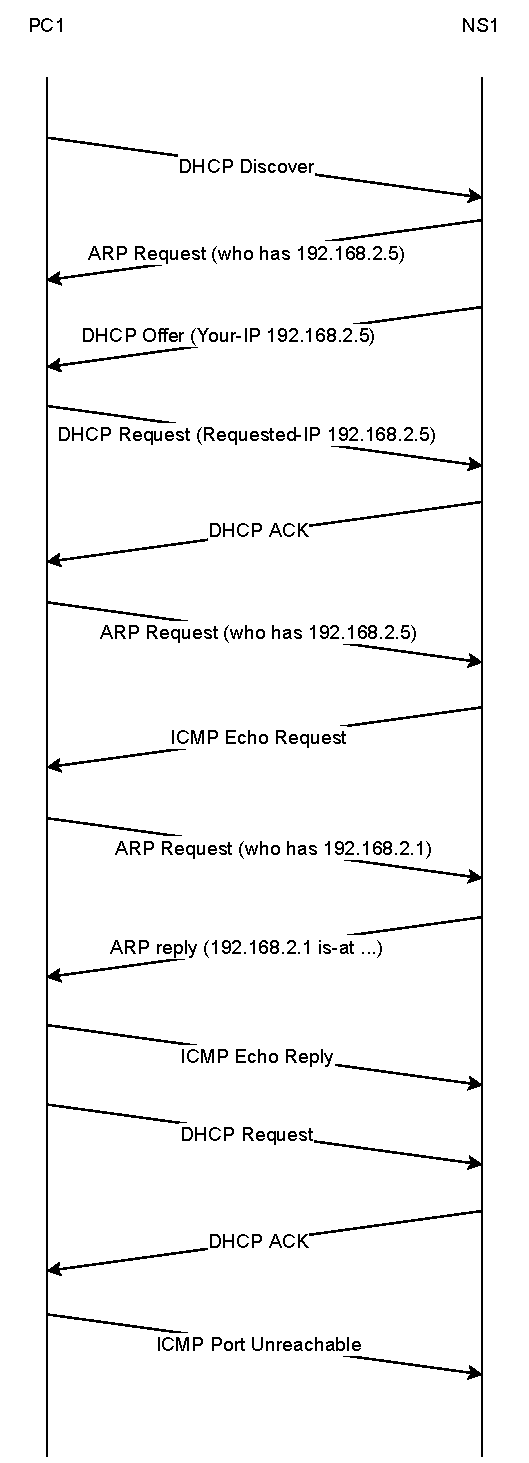
\includegraphics[width=0.5\linewidth]{\imagesPath/1.3.pdf}
			\end{center}
		\end{figure}
		
	\subsection*{1.4}
		Ανταλλάσσονται:
		
		\begin{verbatim}
			DHCPDISCOVER on em0 to 255.255.255.255 
			DHCPDISCOVER on em0 to 255.255.255.255
			DHCPOFFER from 192.168.2.1
			DHCPREQUEST on em0 to 255.255.255.255 
			DHCPACK from 192.168.2.1
		\end{verbatim}
	
	\subsection*{1.5}
		Αποδόθηκε η \verb|192.168.2.5|, ενώ η IP του εξυπηρετητή είναι \verb|192.168.2.1|.
	
	\subsection*{1.6}
		Μετά από 60 δευτερόλεπτα, όπως φαίνεται στη γραμμή:
		
		\begin{verbatim}
			bound to 192.168.2.5 -- renewal in 60 seconds.
		\end{verbatim}
	
	\subsection*{1.7}
		Βλέπουμε ότι χρησιμοποιείται το UDP.
	
	\subsection*{1.8}
		Οι θύρες πηγής και προορισμού είναι οι 67 (PC1) και 68 (NS1).
	
	\subsection*{1.9}
		Έχουμε:
	
		\begin{verbatim}
			Message             Source IP         Destination IP
			DHCP DISCOVER       0.0.0.0           255.255.255.255
			DHCP OFFER          192.168.2.1       192.168.2.5
			DHCP REQUEST        0.0.0.0           255.255.255.255
			DHCP ACK            192.168.2.1       192.168.2.5
		\end{verbatim}
	
	\subsection*{1.10}
		Έχουμε:
		
		\begin{verbatim}
			Message            Source MAC             Destination MAC
			DHCP DISCOVER      08:00:27:cc:ef:48      ff:ff:ff:ff:ff:ff
			DHCP OFFER         08:00:27:64:52:f6      08:00:27:cc:ef:48
			DHCP REQUEST       08:00:27:cc:ef:48      ff:ff:ff:ff:ff:ff
			DHCP ACK           08:00:27:64:52:f6      08:00:27:cc:ef:48
		\end{verbatim}
	
	\subsection*{1.11}
		Μπορεί να το κάνει χρησιμοποιώντας την διεύθυνση IP \verb|0.0.0.0|, τις διευθύνσεις MAC, και την ευρυεκπομπή (όπως φαίνεται στα μηνύματα DHCP DISCOVER/REQUEST).
	
	\subsection*{1.12}
		Ναι, παρατηρήσαμε πλαίσια ARP από τον NS1, ο οποίος θέλει να εξακριβώσει αν χρησιμοποιεί κάποιος τη διεύθυνση IP που σκοπεύει να προσφέρει.
	
	\subsection*{1.13}
		Όχι, δεν παρατηρήσαμε.
	
	\subsection*{1.14}
		Με αυτό το πλαίσιο ARP το PC1 προσπαθεί να επιβεβαιώσει ότι δεν υπάρχει άλλος υπολογιστής με αυτή τη διεύθυνση IP.
	
	\subsection*{1.15}
		Ναι, παρατηρήσαμε ένα ICMP request από τον NS1, και το αντίστοιχο ICMP reply από το PC1. Αυτή η ανταλλαγή γίνεται προκειμένου να επιβεβαιωθεί ότι η απόδοση διεύθυνσης έγινε χωρίς κάποιο πρόβλημα.
	
	\subsection*{1.16}
		Διαρκεί 120 δευτερόλεπτα (\verb|Lease-Time: 120|).
	
	\subsection*{1.17}
		Περιέχει τα επιπλέον options:
		
		\begin{verbatim}
			Server-ID Option 54, length 4: 192.168.2.1
			Requested_IP Option 50, length 4: 192.168.2.5
		\end{verbatim}
	
	\subsection*{1.18}
		Στο δεύτερο DHCP request:
		
		\begin{itemize}
			\item Δεν χρησιμοποιείται πλέον η MAC προορισμού \verb|ff:ff:ff:ff:ff:ff| (broadcast), αλλά η \verb|08:00:27:64:52:f6| (NS1)
			\item Δεν χρησιμοποιείται η IP πηγής \verb|0.0.0.0|, αλλά η \verb|192.168.2.5| (PC1)
			\item Δεν χρησιμοποιείται η IP προορισμού \verb|255.255.255.255| (broadcast), αλλά η \verb|192.168.2.1| (NS1).
			\item Εμφανίζεται το επιπλέον option \verb|"Client IP: 192.168.2.5"|
			\item \textbf{Δεν} εμφανίζεται το option \verb|"Server-ID Option 54, length 4: 192.168.2.1"|.
			\item \textbf{Δεν} εμφανίζεται το option \verb|"Requested-IP Option 50, length 4: 192.168.2.5"|.
		\end{itemize}
	
	\subsection*{1.19} 
		Αυτό συμβαίνει διότι ο πελάτης DHCP (PC1) ανανέωσε τη διεύθυνση IPv4 του, οπότε η σύνδεση στη θύρα 68 δεν χρειάζεται πλέον (σε αντίθεση με αυτή του εξυπηρετητή DHCP στη θύρα 67, που πρέπει να παραμένει ανοιχτή για να ακούσει τυχόν αιτήματα από πελάτες).
	
	\subsection*{1.20}
		Στο αρχείο \verb|/var/db/dhcpd/dhcpd.leases|.
	
	\subsection*{1.21}
		Γίνονται κάθε ένα λεπτό.
	
	\subsection*{1.22}
		Περιέχει τις πληροφορίες:
		
		\begin{verbatim}
			starts ...
			ends ...
			cltt ...
			binding state ...
			next binding state ...
			rewind binding state ...
			hardware ethernet ...
			uid ...
			client-hostname ...
		\end{verbatim}
	
	\subsection*{1.23}
		Στο αρχείο \verb|/var/db/dhclient.leases.em0|.
	
	\subsection*{1.24}
		Περιέχει τις πληροφορίες:
		
		\begin{verbatim}
			interface ...
			fixed-address ...
			option subnet-mask ...
			option routers ...
			option broadcast-address ...
			option dhcp-lease-time ...
			option dhcp-message-type ...
			option dhcp-server-identifier ...
			renew ...
			rebind ...
			expire ...
		\end{verbatim}
		
	\subsection*{1.25}
		Ο ζητούμενος χρόνος είναι ίσος με \verb|rebind - renew = 45 sec|.
	
	\subsection*{1.26}
		Ζήτησε 10 παραμέτρους:
		
		\begin{verbatim}
			Subnet-Mask
			BR
			Time-Zone
			Classless-Static-Route
			Default-Gateway
			Domain-Name
			Domain-Name-Server
			Hostname
			Option 119 (Domain Search List)
			MTU
		\end{verbatim}
	
	\subsection*{1.27}
		Προσδιορίζει τις παραμέτρους \verb|Subnet-Mask, BR|, και  \verb|Default-Gateway|.
	
	\subsection*{1.28}
		Στον NS1 εκτελούμε \verb|tcpdump -ni em0|.
	
	\subsection*{1.29}
		Σε δεύτερη κονσόλα στον NS1 εκτελούμε \verb|service isc-dhcpd stop|.
	
	\subsection*{1.30}
		Στο PC1 εκτελούμε συνεχώς \verb|ifconfig em0| μέχρι η διεπαφή \verb|em0| να μην έχει πλέον διεύθυνση IP. Μόλις συμβεί αυτό, εκτελούμε \verb|service isc-dhcpd start| στον NS1.
	
	\subsection*{1.31}
		Στο PC1 εκτελούμε συνεχώς \verb|ifconfig em0| μέχρι η διεπαφή \verb|em0| να ξαναποκτήσει διεύθυνση IP. Μόλις συμβεί αυτό, σταματάμε την καταγραφή στον NS1.
	
	\subsection*{1.32}
		Στάλθηκαν 4 μηνύματα DHCP:
		
		\begin{verbatim}
			#1 (3 sec) #2 (5 sec) #3 (11 sec) #4 (26 sec) #5			
		\end{verbatim}
	
	\subsection*{1.33}
		Λαμβάνει απάντηση "ICMP udp port 67 unreachable", που σημαίνει ότι ο εξυπηρετητής DHCP δεν ακούει στην θύρα 67, το οποίο είναι λογικό, αφού τον απενεργοποιήσαμε, και έτσι δεν προσφέρεται η υπηρεσία DHCP.
	
	\subsection*{1.34}
		Είναι η διεύθυνση \verb|255.255.255.255| (broadcast).
	
	\subsection*{1.35}
		Χρησιμοποιείται η \verb|255.255.255.255| ως διεύθυνση προορισμού, επειδή αφού λήξει ο χρόνος επανασύνδεσης (rebind), το PC1 προσπαθεί να δανειστεί μία νέα διεύθυνση από οποιονδήποτε άλλο εξυπηρετητή, όχι υποχρεωτικά από αυτόν που δανείστηκε πριν.
	
	\subsection*{1.36}
		Είναι:
		
		\begin{verbatim}
			MAC Destination: ff:ff:ff:ff:ff:ff
			IP Destination: 255.255.255.255
		\end{verbatim}
		
		Το πεδίο του μηνύματος που δείχνει ότι έχει απολεσθεί η διεύθυνση IP είναι το:
		
		\begin{verbatim}
			Requested-IP: 192.168.2.5
		\end{verbatim}
	
	\subsection*{1.37}
		Επειδή ο NS1 προσπαθεί να επιβεβαιώσει ότι δεν χρησιμοποιείται από κάποιον άλλον η διεύθυνση που πρόκειται να προσφέρει.
	
	\subsection*{1.38}
		Στο PC1 εκτελούμε \verb|cat /var/db/dhclient.leases.em0|. Παρατηρούμε ότι με κάθε ανανέωση της IP διεύθυνσης προστίθεται ένα νέο δάνειο στο αρχείο αυτό.
	
	\subsection*{1.39} 
		Αυτό συμβαίνει διότι το DHCP πρέπει να είναι συμβατό με το BOOTP (\href{https://datatracker.ietf.org/doc/html/rfc2131#section-1.6}{RFC 2131}, "DHCP must provide service to existing BOOTP clients") και ως εκ τούτου, ακολουθούνται αυτά που περιγράφονται στο \href{https://datatracker.ietf.org/doc/html/rfc951#section-3}{RFC 951}: \\
			
			We could not simply allow the client to pick a 'random' port number for the UDP source port field; \textbf{since the server reply may be broadcast, a randomly chosen port number could confuse other hosts that happened to be listening on that port.}
			
\section*{Άσκηση 2: Εγκατάσταση εξυπηρετητή DNS}
	
	Εγκαθιστούμε έναν εξυπηρετητή DNS στο NS1:
	
	\subsection*{1.}
		Εκτελούμε \verb|pkg install unbound|.

	\subsection*{2.}
		Εκτελούμε \verb|sysrc unbound_enable="YES"|.

	\subsection*{3.}
		Δημιουργούμε ένα προσωρινό αρχείο \verb|/var/tmp/unbound.conf| με περιεχόμενο: \\
		
		\begin{verbatim}
			server: 
			interface: 0.0.0.0 
			do-ip4: yes 
			do-ip6: yes 
			do-udp: yes 
			do-tcp: yes 
			access-control: 192.168.2.0/24 allow 
			private-domain: "ntua.lab" 
			local-zone: "ntua.lab." static 
			local-data: "ntua.lab. 360 IN SOA ns1.ntua.lab. admin.ntua.lab. 
			                                            20200501 3600 1200 604800 10800" 
			local-data: "ntua.lab. 360 IN NS ns1.ntua.lab." 
			local-data: "ntua.lab. IN MX 10 192.168.2.1" 
			local-data: "ntua.lab. IN A 192.168.2.1" 
			local-data: "ns1.ntua.lab. IN A 192.168.2.1" 
			local-data: "www.ntua.lab. IN CNAME ntua.lab" 
			local-zone: "2.168.192.in-addr.arpa." static 
			local-data-ptr: "192.168.2.1 ns1.ntua.lab." 
			forward-zone: 
			name:"." 
			forward-addr: 1.1.1.1 
			forward-addr: 8.8.8.8 
			forward-addr: 9.9.9.9 
		\end{verbatim}			

	\subsection*{4.}
		Εκτελούμε \verb|unbound-checkconf /var/tmp/unbound.conf|. Δεν υπάρχουν λάθη, οπότε εκτελούμε \verb|cp /var/tmp/unbound.conf /usr/local/etc/unbound/unbound.conf|.

	\subsection*{5.}
		Εκτελούμε \verb|cat /etc/resolv.conf|. Το αρχείο υπάρχει, οπότε εκτελούμε \verb|rm /etc/resolv.conf|. Δημιουργούμε νέο \verb|/etc/resolv.conf| με περιεχόμενα:
		
		\begin{verbatim}
			search ntua.lab
			nameserver 192.168.2.1
		\end{verbatim}

	\subsection*{6.}
		Προσθέτουμε στην αρχή του \verb|/usr/local/etc/dhcpd.conf| τις γραμμές:
		
		\begin{verbatim}
			option domain-name "ntua.lab";
			option domain-name-servers 192.168.2.1;
		\end{verbatim}

	\subsection*{7.}
		Εκτελούμε \verb|service isc-dhcpd restart|. Δεν υπάρχουν λάθη.

	\subsection*{8.}
		Εκτελούμε \verb|poweroff| και ύστερα δημιουργούμε έναν κλώνο του NS1, τον NS2. \\
		
	Πριν ξεκινήσουμε την άσκηση, εκτελούμε:
	
	\begin{verbatim}
		### PC1 ###
		
		ifconfig em0 192.168.2.5/28
		rm /etc/resolv.conf
		
		### PC2 ###
		
		ifconfig em0 192.168.2.6/28
		rm /etc/resolv.conf
	\end{verbatim}
	
	\subsection*{Επίλυση ονομάτων μέσω του αρχείου /etc/hosts}
	
	\subsection*{2.1}
		Στο PC1, τροποποιούμε το \verb|/etc/hosts| ως εξής: (\verb|"---"| σημαίνει διαγραφή γραμμής, ενώ \verb|"+++"| σημαίνει προσθήκη γραμμής):
		
		\begin{verbatim}
			--- ::1               localhost localhost.my.domain
			+++ ::1               localhost localhost.ntua.lab
			
			--- 127.0.0.1         localhost localhost.my.domain
			+++ 127.0.0.1         localhost localhost.ntua.lab
			
			+++ 192.168.2.5       PC1       PC1.ntua.lab
			+++ 192.168.2.6       PC2       PC2.ntua.lab
		\end{verbatim}

	\subsection*{2.2}
		Στο PC1 εκτελούμε:
		
		\begin{verbatim}
			ping PC2
			ping pc2
			ping pc2.NTUA.LAB
		\end{verbatim}
		
		Και στις 3 περιπτώσεις απαντά το PC2, ενώ δεν έχει σημασία η χρήση μικρών ή κεφαλαίων γραμμάτων.
		
	\subsection*{2.3}
		Στο PC2, τροποποιούμε το \verb|/etc/hosts| ως εξής:
		
		\begin{verbatim}
				--- ::1               localhost localhost.my.domain
				+++ ::1               localhost localhost.ntua.lab
				
				--- 127.0.0.1         localhost localhost.my.domain
				+++ 127.0.0.1         localhost localhost.ntua.lab
				
				+++ 192.168.2.5       PC1       PC1.ntua.lab
				+++ 192.168.2.6       PC2       PC2.ntua.lab
		\end{verbatim}
		
		Ύστερα εκτελούμε \verb|ping PC1| και επιβεβαιώνουμε ότι όντως απαντά το PC1.

	\subsection*{2.4}
		Στο PC2 διαγράφουμε την εγγραφή του \verb|/etc/hosts|:
		
		\begin{verbatim}
			192.168.2.5       PC1       PC1.ntua.lab
		\end{verbatim}
		
		Ύστερα εκτελούμε \verb|ping PC1|. Αυτή τη φορά λαμβάνουμε μήνυμα λάθους:
		
		\begin{verbatim}
			ping: cannot resolve PC1: Host name lookup failure
		\end{verbatim}

	\subsection*{Επίλυση ονομάτων μέσω του εξυπηρετητή DNS}

	\subsection*{2.5} 
		Ξεκινάμε τον NS1 και προσθέτουμε στο \verb|/var/tmp/unbound.conf| τις γραμμές:
		
		\begin{verbatim}
			local-data: "PC1.ntua.lab. IN A 192.168.2.5"
			local-data: "PC2.ntua.lab. IN A 192.168.2.6"
		\end{verbatim}

	\subsection*{2.6}
		Στο NS1, στο \verb|/var/tmp/unbound.conf|, προσθέτουμε τις γραμμές:
		
		\begin{verbatim}
			local-data-ptr: "192.168.2.5 PC1.ntua.lab."
			local-data-ptr: "192.168.2.6 PC2.ntua.lab."			
		\end{verbatim}

	\subsection*{2.7}
		Στον NS1 εκτελούμε:
		
		\begin{verbatim}
			unbound-checkconf /var/tmp/unbound.conf      # No errors found.
			cp /var/tmp/unbound.conf /usr/local/etc/unbound/unbound.conf
			service unbound restart
		\end{verbatim}

	\subsection*{2.8}
		Στον NS1 εκτελούμε \verb|tcpdump -vni em0|.

	\subsection*{2.9}
		Στο PC1 εκτελούμε:
		
		\begin{verbatim}
			ifconfig em0 delete
			dhclient em0
		\end{verbatim}

	\subsection*{2.10}
		Σταματάμε την καταγραφή. Το PC1 έλαβε την \verb|192.168.2.5|.

	\subsection*{2.11}
		Απέδωσε επιπλέον τις παραμέτρους \verb|"Domain-Name"| και \verb|"Domain-Name-Server"|.

	\subsection*{2.12}
		Στο PC1 εκτελούμε \verb|cat /etc/resolv.conf|. Το αρχείο έχει δημιουργηθεί και έχει περιεχόμενο:
		
		\begin{verbatim}
			search ntua.lab
			nameserver 192.168.2.1
		\end{verbatim}

	\subsection*{2.13}
		Στο PC1 εκτελούμε:
		
		\begin{verbatim}
			host 192.168.2.5
			
			OR 
			
			drill -x 192.168.2.5
		\end{verbatim}
		
		Στην \verb|192.168.2.5| αντιστοιχεί το όνομα \verb|PC1.ntua.lab|.

	\subsection*{2.14}
		Στο PC1 εκτελούμε \verb|host NS1| και έχουμε:
		
		\begin{verbatim}
			NS1.ntua.lab has address 192.168.2.1
		\end{verbatim}

	\subsection*{2.15}
		Στο PC1 εκτελούμε \verb|ping ns1|. Το ping είναι επιτυχές.

	\subsection*{2.16}
		Στο PC2 εκτελούμε:
		
		\begin{verbatim}
			ifconfig em0 delete
			dhclient em0
		\end{verbatim}

	\subsection*{2.17}
		Έλαβε τη διεύθυνση \verb|192.168.2.6|.

	\subsection*{2.18}
		Στο PC2 εκτελούμε \verb|ping PC1|. Το ping είναι επιτυχές.

	\subsection*{2.19} 
		Την έλαβε από τον εξυπηρετητή DNS, αφού προηγουμένως είχαμε διαγράψει την σχετική εγγραφή του \verb|/etc/hosts| που αφορά το PC1 (ερώτημα 2.4). Μπορούμε να το επιβεβαιώσουμε και στην πράξη, κάνοντας καταγραφή στον NS1 στη διεπαφή \verb|em0| πριν εκτελέσουμε το ping. 

	\subsection*{2.20}
		Στον PC1, αλλάζουμε τη διεύθυνση IP σε \verb|192.168.2.7| στο αρχείο \verb|/etc/hosts| και ύστερα εκτελούμε \verb|ping PC2|. Το ping αποτυγχάνει με μήνυμα λάθους "Host is down".

	\subsection*{2.21}
		Συμπεραίνουμε ότι πρώτα ελέγχεται το αρχείο \verb|/etc/hosts|, και αν δεν υπάρχει σχετική εγγραφή καλείται ο εξυπηρετητής DNS.

	\subsection*{2.22}
		Στο PC1 εκτελούμε \verb|cat /etc/nsswitch.conf|. Είναι:
		
		\begin{verbatim}
			hosts: files dns
		\end{verbatim}
		
		Δηλαδή πρώτα ελέγχεται το αρχείο \verb|/etc/hosts| και ύστερα καλούνται οι εξυπηρετητές DNS. Η σειρά αυτή συμφωνεί με αυτή που είδαμε προηγουμένως.

	\subsection*{2.23}
		Στο PC1 εκτελούμε \verb|host PC2|. Η έξοδος της εντολής είναι:
		
		\begin{verbatim}
			PC2.ntua.lab has address 192.168.2.6
		\end{verbatim}

	\subsection*{2.24}
		Σύμφωνα με την εντολή \verb|man host|, το \verb|host| είναι εργαλείο που εκτελεί DNS lookups, οπότε δεν ασχολείται καθόλου με το περιεχόμενο του αρχείου \verb|/etc/hosts|.

	\subsection*{2.25}
		Στο PC1 εκτελούμε:
		
		\begin{verbatim}
			rm /etc/resolv.conf
			resolvconf -u
			cat /etc/resolv.conf
		\end{verbatim}
		
		Τώρα το περιεχόμενο του \verb|/etc/resolv.conf| είναι:
		
		\begin{verbatim}
			search ntua.lab
			nameserver 192.168.2.1
		\end{verbatim}

	\subsection*{Πρωτόκολλο DNS}

	\subsection*{2.26}
		Στο NS1 εκτελούμε \verb|tcpdump -vni em0 "not port 67 and not port 68"|.

	\subsection*{2.27}
		Στο PC1 εκτελούμε \verb|host ntua.lab|.

	\subsection*{2.28}
		Ναι, υπάρχει.

	\subsection*{2.29}
		Χρησιμοποιήθηκε το UDP.

	\subsection*{2.30}
		Οι θύρες προέλευσης και προορισμού είναι οι 53, 16104, 21507 και 45142.

	\subsection*{2.31}
		Η θύρα 53.

	\subsection*{2.32}
		Στο NS1 εκτελούμε \verb|tcpdump -vni em0 "udp port 53"|.

	\subsection*{2.33}
		Στο PC1 εκτελούμε \verb|host NS1|.

	\subsection*{2.34}
		Ανταλλάχθηκαν 6 μηνύματα.

	\subsection*{2.35}
		Αντιστοιχούσαν σε ερωτήματα είδους \verb|A|, \verb|AAAA| και \verb|MX| για το όνομα \verb|NS1.ntua.lab|.

	\subsection*{2.36}
		Δόθηκε απάντηση μόνο στο ερώτημα είδους \verb|A| (δηλαδή για την διεύθυνση IPv4).

	\subsection*{2.37}
		Στο PC1 εκτελούμε:
		
		\begin{verbatim}
			drill ns1
			drill ns1.ntua.lab
		\end{verbatim}

	\subsection*{2.38}
		Έγιναν οι ερωτήσεις για τα ονόματα:
		
		\begin{verbatim}
			### drill ns1 ###
			---> name: ns1
			
			### drill ns1.ntua.lab ###
			---> name: ns1.ntua.lab
		\end{verbatim} 
		
		και λήφθηκαν οι απαντήσεις:
		
		\begin{verbatim}
			### drill ns1 ###
			---> <no answer>
			
			### drill ns1.ntua.lab ###
			---> ns1.ntua.lab.   3600    IN      A       192.168.2.1
		\end{verbatim}

	\subsection*{2.39}
		Συμπεραίνουμε ότι στην εντολή \verb|host| δεν απαιτείται η χρήση του επιθέματος \verb|ntua.lab|, ενώ στην εντολή \verb|drill| χρειάζεται.

	\subsection*{2.40}
		Στο PC1 εκτελούμε:
		
		\begin{verbatim}
			ping localhost
			ping pc1
		\end{verbatim}
		
		Δεν παράγονται ερωτήσεις προς τον εξυπηρετητή DNS σε καμία περίπτωση.

	\subsection*{2.41}
		Στο PC1 εκτελούμε \verb|ping -c 1 ns1|.

	\subsection*{2.42}
		Ανταλλάχθηκαν 2 μηνύματα DNS, που αφορούσαν το ερώτημα \verb|A? ns1.ntua.lab|, δηλαδή είδους \verb|A| (IPv4 διεύθυνση) για το όνομα \verb|ns1.ntua.lab|.  

	\subsection*{2.43}
		Στο PC1 εκτελούμε:
		
		\begin{verbatim}
			ping -c 1 ns1
			ping -c 1 ns1
			ping -c 1 ns1
		\end{verbatim}
		
		Παρατηρούμε να παράγονται 3 επιπλέον ερωτήματα προς τον εξυπηρετητή DNS, όσα και τα ping που εκτελέσαμε.

	\subsection*{2.44}
		Συμπεραίνουμε ότι οι απαντήσεις του εξυπηρετητή DNS δεν αποθηκεύονται προσωρινά στο PC1.

\section*{Άσκηση 3: Εγκατάσταση εξυπηρετητή HTTP}
	
	Για την εγκατάσταση του εξυπηρετητή HTTP στον SRV κάνουμε τα εξής:
	
	\subsection*{1.}
		Επιβεβαιώνουμε ότι η διεπαφή \verb|em1| είναι σε NAT.
		
	\subsection*{2.}
		Εκτελούμε \verb|dhclient em1|.

	\subsection*{3.}
		Εκτελούμε \verb|ping www.google.com|. Το ping είναι επιτυχές.

	\subsection*{4.}
		Εκτελούμε \verb|pkg install lighttpd|.

	\subsection*{5.}
		Απενεργοποιούμε τις διεπαφές πλην της \verb|em0| και εκτελούμε \verb|rm /etc/resolv.conf|.
			
	\subsection*{3.1}
		Στον SRV εκτελούμε:
		
		\begin{verbatim}
			sysrc hostname="SRV"
			sysrc lighttpd_enable="YES"
		\end{verbatim}

	\subsection*{3.2}
		Στον SRV εκτελούμε:
		
		\begin{verbatim}
			mkdir /usr/local/www/data
		\end{verbatim}

	\subsection*{3.3}
		Στον SRV εκτελούμε:
		
		\begin{verbatim}
			echo "Hello World!" > /usr/local/www/data/index.html
		\end{verbatim}

	\subsection*{3.4}
		Στον SRV εκτελούμε:
		
		\begin{verbatim}
			reboot
			rm /etc/resolv.conf
		\end{verbatim}

	\subsection*{3.5}
		Μπορούμε να εκτελέσουμε \verb|service lighttpd status|.

	\subsection*{3.6}
		Μπορούμε να εκτελέσουμε την εντολή \verb+netstat -an | grep 80+ ή την \verb+netstat -a | grep http+. Αν υπάρχει εξυπηρετητής http θα εμφανιστεί έξοδος της μορφής:
		
		\begin{verbatim}
			tcp6    0    0    *.http            *.*            LISTEN
			tcp4    0    0    *.http            *.*            LISTEN
		\end{verbatim}

	\subsection*{3.7}
		Τοποθετούμε τη διεπαφή \verb|em0| του SRV στο LAN1 και ύστερα εκτελούμε:
		
		\begin{verbatim}
			ifconfig em0 192.168.2.3/28
		\end{verbatim}

	\subsection*{3.8}
		Στο \verb|/var/tmp/unbound.conf| του NS1 προσθέτουμε τη γραμμή:
		
		\begin{verbatim}
			local-data: "SRV.ntua.lab. IN A 192.168.2.3"
		\end{verbatim}
		
	\subsection*{3.9}
		Στο \verb|/var/tmp/unbound.conf| του NS1 προσθέτουμε τη γραμμή:
		
		\begin{verbatim}
			local-data-ptr: "192.168.2.3 SRV.ntua.lab."
		\end{verbatim}

	\subsection*{3.10}
		Στον NS1 εκτελούμε:
		
		\begin{verbatim}
			unbound-checkconf /var/tmp/unbound.conf   # No errors found.
			cp /var/tmp/unbound.conf /usr/local/etc/unbound/unbound.conf
			service unbound restart
		\end{verbatim}

	\subsection*{3.11}
		Στον SRV εκτελούμε \verb|tcpdump -ni em0|.

	\subsection*{3.12}
		Στο PC1 εκτελούμε \verb|fetch http://srv.ntua.lab|.

	\subsection*{3.13}
		Χρησιμοποιήθηκε το TCP, ενώ ο εξυπηρετητής http ακούει στη θύρα 80.
		
	\subsection*{3.14}
		Αποθηκεύτηκε στο \verb|srv.ntua.lab|.
		
\section*{Άσκηση 4: Εγκατάσταση ιδιωτικού δρομολογητή και Firewall}

	\subsection*{4.1}
		Στον NS1 εκτελούμε \verb|sysrc gateway_enable="YES"|.

	\subsection*{4.2}
		Στον NS1 εκτελούμε \verb|sysrc firewall_enable="YES"|.

	\subsection*{4.3}
		Στον NS1 εκτελούμε \verb|sysrc firewall_type="open"|.

	\subsection*{4.4}
		Στον NS1 εκτελούμε \verb|sysrc firewall_nat_enable="YES"|.

	\subsection*{4.5}
		Στον NS1 εκτελούμε \verb|sysrc ifconfig_em2="192.168.2.17/28"|.

	\subsection*{4.6}
		Στον NS1 εκτελούμε:
		
		\begin{verbatim}
			cat /etc/rc.conf        # Everything OK.
		\end{verbatim}

	\subsection*{4.7}
		Στο NS1 εκτελούμε \verb|poweroff|, τοποθετούμε τη διεπαφή \verb|em2| του NS1 στο DMZ και το επανεκκινούμε. Ύστερα εκτελούμε \verb|netstat -rn| και βλέπουμε ότι η προκαθορισμένη πύλη είναι σωστά ρυθμισμένη. 
		
	\subsection*{4.8} 
		Στο NS1 εκτελούμε \verb|vi /etc/resolv.conf| και αλλάζουμε τα περιεχόμενα του αρχείου σε:
		
		\begin{verbatim}
			search ntua.lab
			nameserver 192.168.2.1
		\end{verbatim}
		
		Επιβεβαιώνουμε ότι η επίλυση ονομάτων λειτουργεί.

	\subsection*{4.9}
		Στο PC1 εκτελούμε:
		
		\begin{verbatim}
			sysrc ifconfig_em0="DHCP"
			service netif restart
		\end{verbatim} 

	\subsection*{4.10}
		Στο PC2 εκτελούμε:
		
		\begin{verbatim}
			sysrc ifconfig_em0="192.168.2.4/28"
			sysrc defaultrouter="192.168.2.1"
		\end{verbatim}

	\subsection*{4.11}
		Στο PC2 εκτελούμε:
		
		\begin{verbatim}
			service netif restart
			service routing restart
			vi /etc/resolv.conf
		\end{verbatim}
		
		Αλλάζουμε το περιεχόμενο του \verb|/etc/resolv.conf| σε:
		
		\begin{verbatim}
			nameserver 192.168.2.1
		\end{verbatim}
		
		Τέλος επιβεβαιώνουμε ότι η επίλυση ονομάτων λειτουργεί με οποιαδήποτε από τις παρακάτω εντολές:
		
		\begin{verbatim}
			ping PC1     
			---> Successful
			
			host PC1.ntua.lab 
			---> PC1.ntua.lab has address 192.168.2.5
			
			host 192.168.2.5
			---> 5.2.168.192.in-addr.arpa domain name pointer PC1.ntua.lab
		\end{verbatim}

	\subsection*{4.12}
		Τοποθετούμε την διεπαφή \verb|em0| του SRV στο τοπικό δίκτυο DMZ και ύστερα στον SRV εκτελούμε:
		
		\begin{verbatim}
			sysrc ifconfig_em0="192.168.2.18/28"
			sysrc defaultrouter="192.168.2.17"
			service netif restart
			service routing restart
		\end{verbatim}

	\subsection*{4.13}
		Στον NS1 εκτελούμε \verb|vi /var/tmp/unbound.conf| και διορθώνουμε τις γραμμές \\ (\verb|"---"| $\rightarrow$ παλιά γραμμή, \verb|"+++"| $\rightarrow$ καινούργια γραμμή):
		
		\begin{verbatim}
			--- local-data: "PC2.ntua.lab. IN A 192.168.2.6"
			+++ local-data: "PC2.ntua.lab. IN A 192.168.2.4"
			
			--- local-data: "SRV.ntua.lab. IN A 192.168.2.3"
			+++ local-data: "SRV.ntua.lab. IN A 192.168.2.18"
			
			--- local-data-ptr: "192.168.2.6 PC2.ntua.lab."
			+++ local-data-ptr: "192.168.2.4 PC2.ntua.lab."
			
			--- local-data-ptr: "192.168.2.3 SRV.ntua.lab."
			+++ local-data-ptr: "192.168.2.18 SRV.ntua.lab."
		\end{verbatim}
		
		Ύστερα εκτελούμε:
		
		\begin{verbatim}
			unbound-checkconf /var/tmp/unbound.conf      # No errors found.
			cp /var/tmp/unbound.conf /usr/local/etc/unbound/unbound.conf
			service unbound restart
		\end{verbatim}

	\subsection*{4.14}
		Στον SRV εκτελούμε:
		
		\begin{verbatim}
			ping 192.168.2.5   # PC1
			ping 192.168.2.4   # PC2 
			ping 192.168.2.1   # NS1
		\end{verbatim}
		
		Ναι, μπορούμε να κάνουμε ping στα μηχανήματα του LAN1 χρησιμοποιώντας την IP διεύθυνσή τους.

	\subsection*{4.15}
		Στο NS1 εκτελούμε:
		
		\begin{verbatim}
			ipfw add 2000 deny all from any to 192.168.2.0/28 in via em2
		\end{verbatim}

	\subsection*{4.16}
		Στον SRV εκτελούμε \verb|ping 192.168.2.5|. Δεν λαμβάνουμε απάντηση.
		
	\subsection*{4.17} 
		Στον NS1 εκτελούμε (όλο μαζί μία εντολή):
		
		\begin{verbatim}
			ipfw add 1900 allow all from 192.168.2.0/28 to 192.168.2.16/28 \
			in recv em0 keep-state
		\end{verbatim}

	\subsection*{4.18}
		Στο PC1 εκτελούμε \verb|ping SRV|. Το ping είναι επιτυχές.

	\subsection*{4.19}
		Στο NS1 εκτελούμε \verb|ping 147.102.1.1|. Το ping είναι επιτυχές.

	\subsection*{4.20}
		Στο PC1 εκτελούμε \verb|ping 147.102.1.1|. Δεν λαμβάνουμε απάντηση.

	\subsection*{4.21}
		Στον NS1 εκτελούμε:
		
		\begin{verbatim}
			ipfw nat 111 config unreg_only if em1 reset
		\end{verbatim}

	\subsection*{4.22}
		Στον NS1 εκτελούμε:
		
		\begin{verbatim}
			ipfw add 3000 nat 111 ip4 from any to any via em1 
		\end{verbatim}

	\subsection*{4.23}
		Στο PC1 εκτελούμε \verb|ping 147.102.1.1|. Το ping είναι επιτυχές.

	\subsection*{4.24}
		Στο PC1 εκτελούμε \verb|host 147.102.1.1|. Το όνομα του μηχανήματος με αυτή τη διεύθυνση IP είναι \verb|theseas.softlab.ece.ntua.gr|.

	\subsection*{4.25}
		Στον NS1 εκτελούμε \verb|tcpdump -ni em1|.

	\subsection*{4.26}
		Στο PC1 εκτελούμε \verb|ping -c 2 www.ntua.gr|. Τα πακέτα που παράγει το PC1 εμφανίζονται με διεύθυνση πηγής \verb|10.0.3.15|.

	\subsection*{4.27}
		Είναι η \verb|147.102.224.101|.

	\subsection*{4.28}
		Έγινε προς τον \verb|9.9.9.9 (dns9.quad9.net)|.

	\subsection*{4.29}
		Στον NS1 εκτελούμε \verb|tcpdump -ni em1 "udp port 53"|.

	\subsection*{4.30}
		Στο PC2 εκτελούμε:
		
		\begin{verbatim}
			#1: ping -c 1 www.google.com
			#2: ping -c 1 www.cnn.com
			#3: ping -c 1 www.yahoo.com
			#4: ping -c 1 www.mit.edu
		\end{verbatim}
		
		Κάθε φορά καλείται ένας εξυπηρετητής από αυτούς που έχουμε ορίσει, δηλαδή \verb|1.1.1.1, 8.8.8.8| και \verb|9.9.9.9|.

	\subsection*{4.31}
		Σε νέο παράθυρο στον NS1 εκτελούμε \verb|tcpdump -ni em0 "udp port 53"|.

	\subsection*{4.32}
		Στο PC1 εκτελούμε \verb|ping -c 1 courses.cn.ntua.gr|. Το canonical name του \verb|courses.cn.ntua.gr| είναι \verb|courses.cn.ece.ntua.gr|.

	\subsection*{4.33}
		Το PC1 έκανε ερώτημα \verb|"A"|:
		
		\begin{verbatim}
			A? courses.cn.ntua.gr.
		\end{verbatim}
		
		και έλαβε απάντηση \verb|"CNAME", "A"| από τον NS1:
		
		\begin{verbatim}
			CNAME courses.cn.ece.ntua.gr, A 147.102.40.10
		\end{verbatim}

		Επίσης, ο NS1 έκανε ερωτήματα είδους \verb|"A"| στους εξωτερικούς εξυπηρετητές DNS:
		
		\begin{verbatim}
			#1   A? courses.cn.ntua.gr.
			#2   A? courses.cn.ece.ntua.gr
		\end{verbatim} 
		
		και έλαβε απαντήσεις είδους \verb|"CNAME", "A"| και \verb|"A"| αντίστοιχα:
		
		\begin{verbatim}
			#1   CNAME courses.cn.ece.ntua.gr, A 147.102.40.10
			#2   A 147.102.40.10
		\end{verbatim}

	\subsection*{4.34}
		Στον NS1 εκτελούμε \verb|tcpdump -vvvni em1 "udp port 53"|.

	\subsection*{4.35} 
		Στο PC1 εκτελούμε:
		
		\begin{verbatim}
			drill www.cn.ece.ntua.gr
			drill www.cn.ece.ntua.gr
		\end{verbatim}

		Παρατηρήσαμε μόνο ένα ερώτημα DNS:
		
		\begin{verbatim}
			A? www.cn.ece.ntua.gr
		\end{verbatim}
		
		Οι απαντήσεις DNS ισχύουν για 20 λεπτά.
		
	\subsection*{4.36}
		Στον NS1 εκτελούμε \verb|tcpdump -vvvni em0 "udp port 53"|. Ύστερα στο PC1 εκτελούμε:
		
		\begin{verbatim}
			drill www.cn.ece.ntua.gr
			drill www.cn.ece.ntua.gr
		\end{verbatim}
		
		Παράγονται μηνύματα DNS κάθε φορά που εκτελούμε την εντολή \verb|drill|. Παρατηρούμε ότι η χρονική διάρκεια ισχύος των απαντήσεων DNS μειώνεται συνεχώς.

	\subsection*{4.37}
		Συμπεραίνουμε ότι οι απαντήσεις που λαμβάνει ο τοπικός εξυπηρετητής DNS στο NS1 αποθηκεύονται προσωρινά.

	\subsection*{4.38}
		Στον SRV εκτελούμε \verb|ping 147.102.224.101|. Το ping είναι επιτυχές.

	\subsection*{4.39}
		Στον SRV εκτελούμε \verb|ping www.ntua.gr|. Το ping αποτυγχάνει με μήνυμα λάθους:
		
		\begin{verbatim}
			ping: cannot resolve www.ntua.gr: Host name lookup failure
		\end{verbatim}
		
		Αυτό συμβαίνει διότι:
		
		\begin{itemize}
			\item Δεν υπάρχει εγγραφή σχετική με τον \verb|www.ntua.gr| στο αρχείο \verb|/etc/hosts|.
			\item Δεν έχει οριστεί εξυπηρετητής DNS, αφού δεν υπάρχει το αρχείο \verb|/etc/resolv.conf|.
		\end{itemize}

	\subsection*{4.40}
		Στον SRV εκτελούμε:
		
		\begin{verbatim}
			echo "nameserver 192.168.2.17" > /etc/resolv.conf
		\end{verbatim}

	\subsection*{4.41}
		Στον SRV εκτελούμε \verb|ping www.ntua.gr|. Το ping είναι επιτυχές.

	\subsection*{4.42}
		Στο PC1 εκτελούμε \verb|host www.ntua.lab| και παίρνουμε την απάντηση:
		
		\begin{verbatim}
			www.ntua.lab is an alias for ntua.lab
		\end{verbatim}
		
		Για να πάρουμε τη διεύθυνση IP πρέπει να ξαναεκτελέσουμε την \verb|host|, αλλά αυτή τη φορά να βάλουμε σαν όρισμα την έξοδο του προηγούμενου \verb|host|, δηλαδή:
		
		\begin{verbatim}
			host ntua.lab
		\end{verbatim}
		
		Οπότε παίρνουμε ως απάντηση τη διεύθυνση \verb|192.168.2.1|. \\
		
		Στο PC1 εκτελούμε \verb|ping www.ntua.lab|. Το ping αποτυγχάνει με μήνυμα λάθους:
		
		\begin{verbatim}
			ping: cannot resolve www.ntua.lab: Unknown server error
		\end{verbatim}

	\subsection*{4.43}
		Στον NS1 εκτελούμε \verb|vi /usr/local/etc/unbound/unbound.conf| και προσθέτουμε πριν από την εγγραφή CNAME τη γραμμή:
		
		\begin{verbatim}
			local-data: "www.ntua.lab. IN A 192.168.2.18"
		\end{verbatim}
		
		Ύστερα εκτελούμε \verb|service unbound restart|.

	\subsection*{4.44}
		Στο PC1 εκτελούμε \verb|ping www.ntua.lab|. Απαντά το SRV (\verb|192.168.2.18|).

\section*{Άσκηση 5: Εγκατάσταση δημόσιου δρομολογητή και DNS}
	
	Πριν ξεκινήσουμε, τοποθετούμε τις διεπαφές του NS2 ως εξής:
	
	\begin{verbatim}
		em0: LAN2
		em1: NAT
		em2: WAN
	\end{verbatim}

	\subsection*{5.1}
		Στον NS2 εκτελούμε \verb|sysrc hostname="ns2.ntua.lab"|.

	\subsection*{5.2}
		Στον NS2 εκτελούμε:
		
		\begin{verbatim}
			sysrc ifconfig_em0="192.0.2.1/29"
			sysrc ifconfig_em2="192.0.2.9/29"
		\end{verbatim}

	\subsection*{5.3}
		Στον NS2 εκτελούμε \verb|sysrc ifconfig_em1="DHCP"|.

	\subsection*{5.4}
		Στον NS2 εκτελούμε \verb|sysrc gateway_enable="YES"|.

	\subsection*{5.5}
		Στον NS2 εκτελούμε \verb|sysrc firewall_enable="YES"|.

	\subsection*{5.6}
		Στον NS2 εκτελούμε \verb|sysrc firewall_type="open"|.

	\subsection*{5.7}
		Στον NS2 εκτελούμε \verb|sysrc firewall_nat_enable="YES"|.

	\subsection*{5.8}
		Στον NS2 εκτελούμε:
		
		\begin{verbatim}
			sysrc -a     # To see DHCP server related settings
			
			# DHCP server related:
			# dhcp_ifaces
			# dhcpd_enable
			
			sysrc -x dhcp_ifaces
			sysrc -x dhcpd_enable
		\end{verbatim}

	\subsection*{5.9}
		Στον NS2 εκτελούμε \verb|sysrc -a|. Επιβεβαιώνουμε ότι υπάρχει (\verb|unbound_enable: YES|).

	\subsection*{5.10}
		Στον NS2 εκτελούμε \verb|vi /var/tmp/unbound.conf| και αλλάζουμε τις γραμμές \\ (\verb|"---"| $\rightarrow$ γραμμή που διαγράφηκε, \verb|"+++"| $\rightarrow$ γραμμή που προστέθηκε):
		
		\begin{verbatim}
			### NTUA.LAB RELATED LINES ###
		
			--- private-domain: "ntua.lab"
			--- local-zone: "ntua.lab." static
			--- local-data: "ntua.lab. 360 IN SOA ns1.ntua.lab. admin.ntua.lab. 
			                                      20200501 3600 1200 604800 10800"
			--- local-data: "ntua.lab. 360 IN NS ns1.ntua.lab."
			--- local-data: "ntua.lab. IN MX 10 192.168.2.1"
			--- local-data: "ntua.lab. IN A 192.168.2.1"
			--- local-data: "ns1.ntua.lab. IN A 192.168.2.1"
			--- local-data: "www.ntua.lab. IN CNAME ntua.lab."
			--- local-data-ptr: "192.168.2.1 ns1.ntua.lab."
			
			### ACCESS-CONTROL ###
			
			--- access-control: 192.168.2.0/24 allow
			
			### NEW LINES ###
			
			+++ access-control: 192.0.2.0/24 allow
			+++ local-zone: "ntua.lab." redirect
			+++ local-data: "ntua.lab. IN A 192.0.2.10"
		\end{verbatim}

		Ύστερα εκτελούμε:
		
		\begin{verbatim}
			unbound-checkconf /var/tmp/unbound.conf    # No errors found.
			cp /var/tmp/unbound.conf /usr/local/etc/unbound/unbound.conf			
		\end{verbatim}

	\subsection*{5.11} 
		Στον NS2 εκτελούμε:
		
		\begin{verbatim}
			reboot
			netstat -rn     #  default gateway exists, OK.
		\end{verbatim}

	\subsection*{5.12}
		Στον NS2 εκτελούμε:
		
		\begin{verbatim}
			ipfw nat 222 config if em1 reset same_ports
		\end{verbatim}

	\subsection*{5.13}
		Στον NS2 εκτελούμε:
		
		\begin{verbatim}
			ipfw add 1100 nat 222 ip4 from any to any via em1
		\end{verbatim}

	\subsection*{5.14}
		Στο PC2 εκτελούμε:
		
		\begin{verbatim}
			sysrc ifconfig_em0="192.0.2.2/29"
			sysrc defaultrouter="192.0.2.1"
		\end{verbatim}

	\subsection*{5.15}
		Συνδέουμε το PC2 στο LAN2 και εκτελούμε:
		
		\begin{verbatim}
			service netif restart
			service routing restart
			echo "nameserver 192.0.2.1" > /etc/resolv.conf
			host google.com              # Name resolution OK.
		\end{verbatim}

	\subsection*{5.16}
		Στο PC2 εκτελούμε \verb|www.ntua.gr|. Το ping είναι επιτυχές.
	
	\subsection*{5.17}
		Στον NS1 εκτελούμε:
		
		\begin{verbatim}
			sysrc ifconfig_em1="192.0.2.10/29"
			sysrc defaultrouter="192.0.2.9"
		\end{verbatim}
		
	\subsection*{5.18}
		Μετακινούμε την \verb|em1| του NS1 στο WAN και ύστερα εκτελούμε:
		
		\begin{verbatim}
			service netif restart
			service routing restart
		\end{verbatim}

	\subsection*{5.19}
		Εκτελούμε:
		
		\begin{verbatim}
			### NS1 ###
			ipfw zero
		
			### PC1 ###
			ping www.ntua.gr 
			
			### NS1 ###
			ipfw show          # NAT 111 rule used
			ipfw zero
			
			### SRV ###
			ping www.ntua.gr
			
			### NS1 ###
			ipfw show          # NAT 111 rule used
		\end{verbatim}
		
		Και τα δύο ping είναι επιτυχή, ενώ παραμένει η λειτουργία του πίνακα nat 111.

	\subsection*{5.20}
		Εκτελούμε:
		
		\begin{verbatim}
			### PC1 ###
			host www.ntua.lab
			
			### PC2 ###
			host www.ntua.lab
		\end{verbatim}
		
		Στο PC1 δίνει διεύθυνση \verb|192.168.2.18|, ενώ στο PC2 \verb|192.0.2.10|.

	\subsection*{5.21}
		Στο PC2 εκτελούμε \verb|fetch http://www.ntua.lab|. Η εντολή αποτυγχάνει με μήνυμα λάθους "Connection refused".
	
	\subsection*{5.22}
		Στον NS1 εκτελούμε:
		
		\begin{verbatim}
			ipfw nat 111 config unreg_only if em1 reset redirect_port tcp 192.168.2.18:80 80
		\end{verbatim}

	\subsection*{5.23}
		Στο PC2 εκτελούμε \verb|fetch http://www.ntua.lab|. Πλέον μπορούμε να κατεβάσουμε κανονικά την ιστοσελίδα.

	\subsection*{5.24}
		Στο PC2 εκτελούμε \verb|ping www.ntua.lab|. Απαντά το NS1 \verb|(192.0.2.10)|.

	\subsection*{5.25}
		Στο PC1 εκτελούμε \verb|ssh lab@www.ntua.lab|. Συνδεόμαστε στο SRV, όπως φαίνεται και από το prompt.

	\subsection*{5.26}
		Στο PC2 εκτελούμε \verb|ssh lab@www.ntua.lab|. Συνδεόμαστε στο μηχάνημα NS1 (όπως φαίνεται από το prompt), αφού στο PC2 το όνομα \verb|www.ntua.lab| αντιστοιχεί στη διεύθυνση \verb|192.0.2.10|, όπως μπορούμε να επιβεβαιώσουμε και με την εντολή \verb|host www.ntua.lab|.

	\subsection*{5.27}
		Στο NS1 εκτελούμε (όλο μαζί μία εντολή):
		
		\begin{verbatim}
			ipfw nat 111 config unreg_only if em1 reset \
			redirect_port tcp 192.168.2.18:80 80        \
			redirect_port tcp 192.168.2.18:22 22
		\end{verbatim}

	\subsection*{5.28}
		Στο PC2 εκτελούμε \verb|ssh lab@www.ntua.lab|. Συνδεόμαστε στον SRV, όπως μπορούμε να επιβεβαιώσουμε από το prompt, την εντολή \verb|hostname|, ή -αν θέλουμε να είμαστε απολύτως σίγουροι- διασταυρώνοντας τις διευθύνσεις MAC στην έξοδο της \verb|ifconfig|.
	
\end{document}
